\subsection{Umsetzung}

Neben den o.g. Betrachtungen zur theoretischen Erarbeitung des linearen Algorithmus ist ein weiterer Bestandteil meiner Komplexen Leistung die praktische Umsetzung. Aufgrund des limitierten Umfangs der Komplexen Leistung kann ich nur sehr kurz auf die Implementierung des Algorithmus eingehen.
Der Code ist ausschließlich in Python geschrieben. Er ist öffentlich auf Github zugänglich und dort auch ausführlich dokumentiert \cite{implementierung}. 

Sowohl die theoretische Erarbeitung des Algorithmus, als auch die Implementierung des Algorithmus habe ich zusammen mit Max Polter erarbeitet. Dabei habe ich den gesamten Code des Winkel- und Orientierungstest geschrieben, sowie Teile des Kanalpolygons und der Chokepointsuche. Den Algorithmus haben wir in großen Teilen zusammen erarbeitet. Er kann alle Beispielaufgaben des 43. Bundeswettbewerb Informatik lösen \cite{beispielaufgaben}. In den folgenden Abbildungen (\hyperref[fig:beispiele]{Abb. 13}) und (\hyperref[fig:beispiele2]{Abb. 14}) werden die Ergebnisse des Algorithmus dargestellt.

\begin{figure}[h]
\label{fig:beispiele}
     \centering
     \begin{subfigure}[b]{0.49\textwidth}
         \centering
         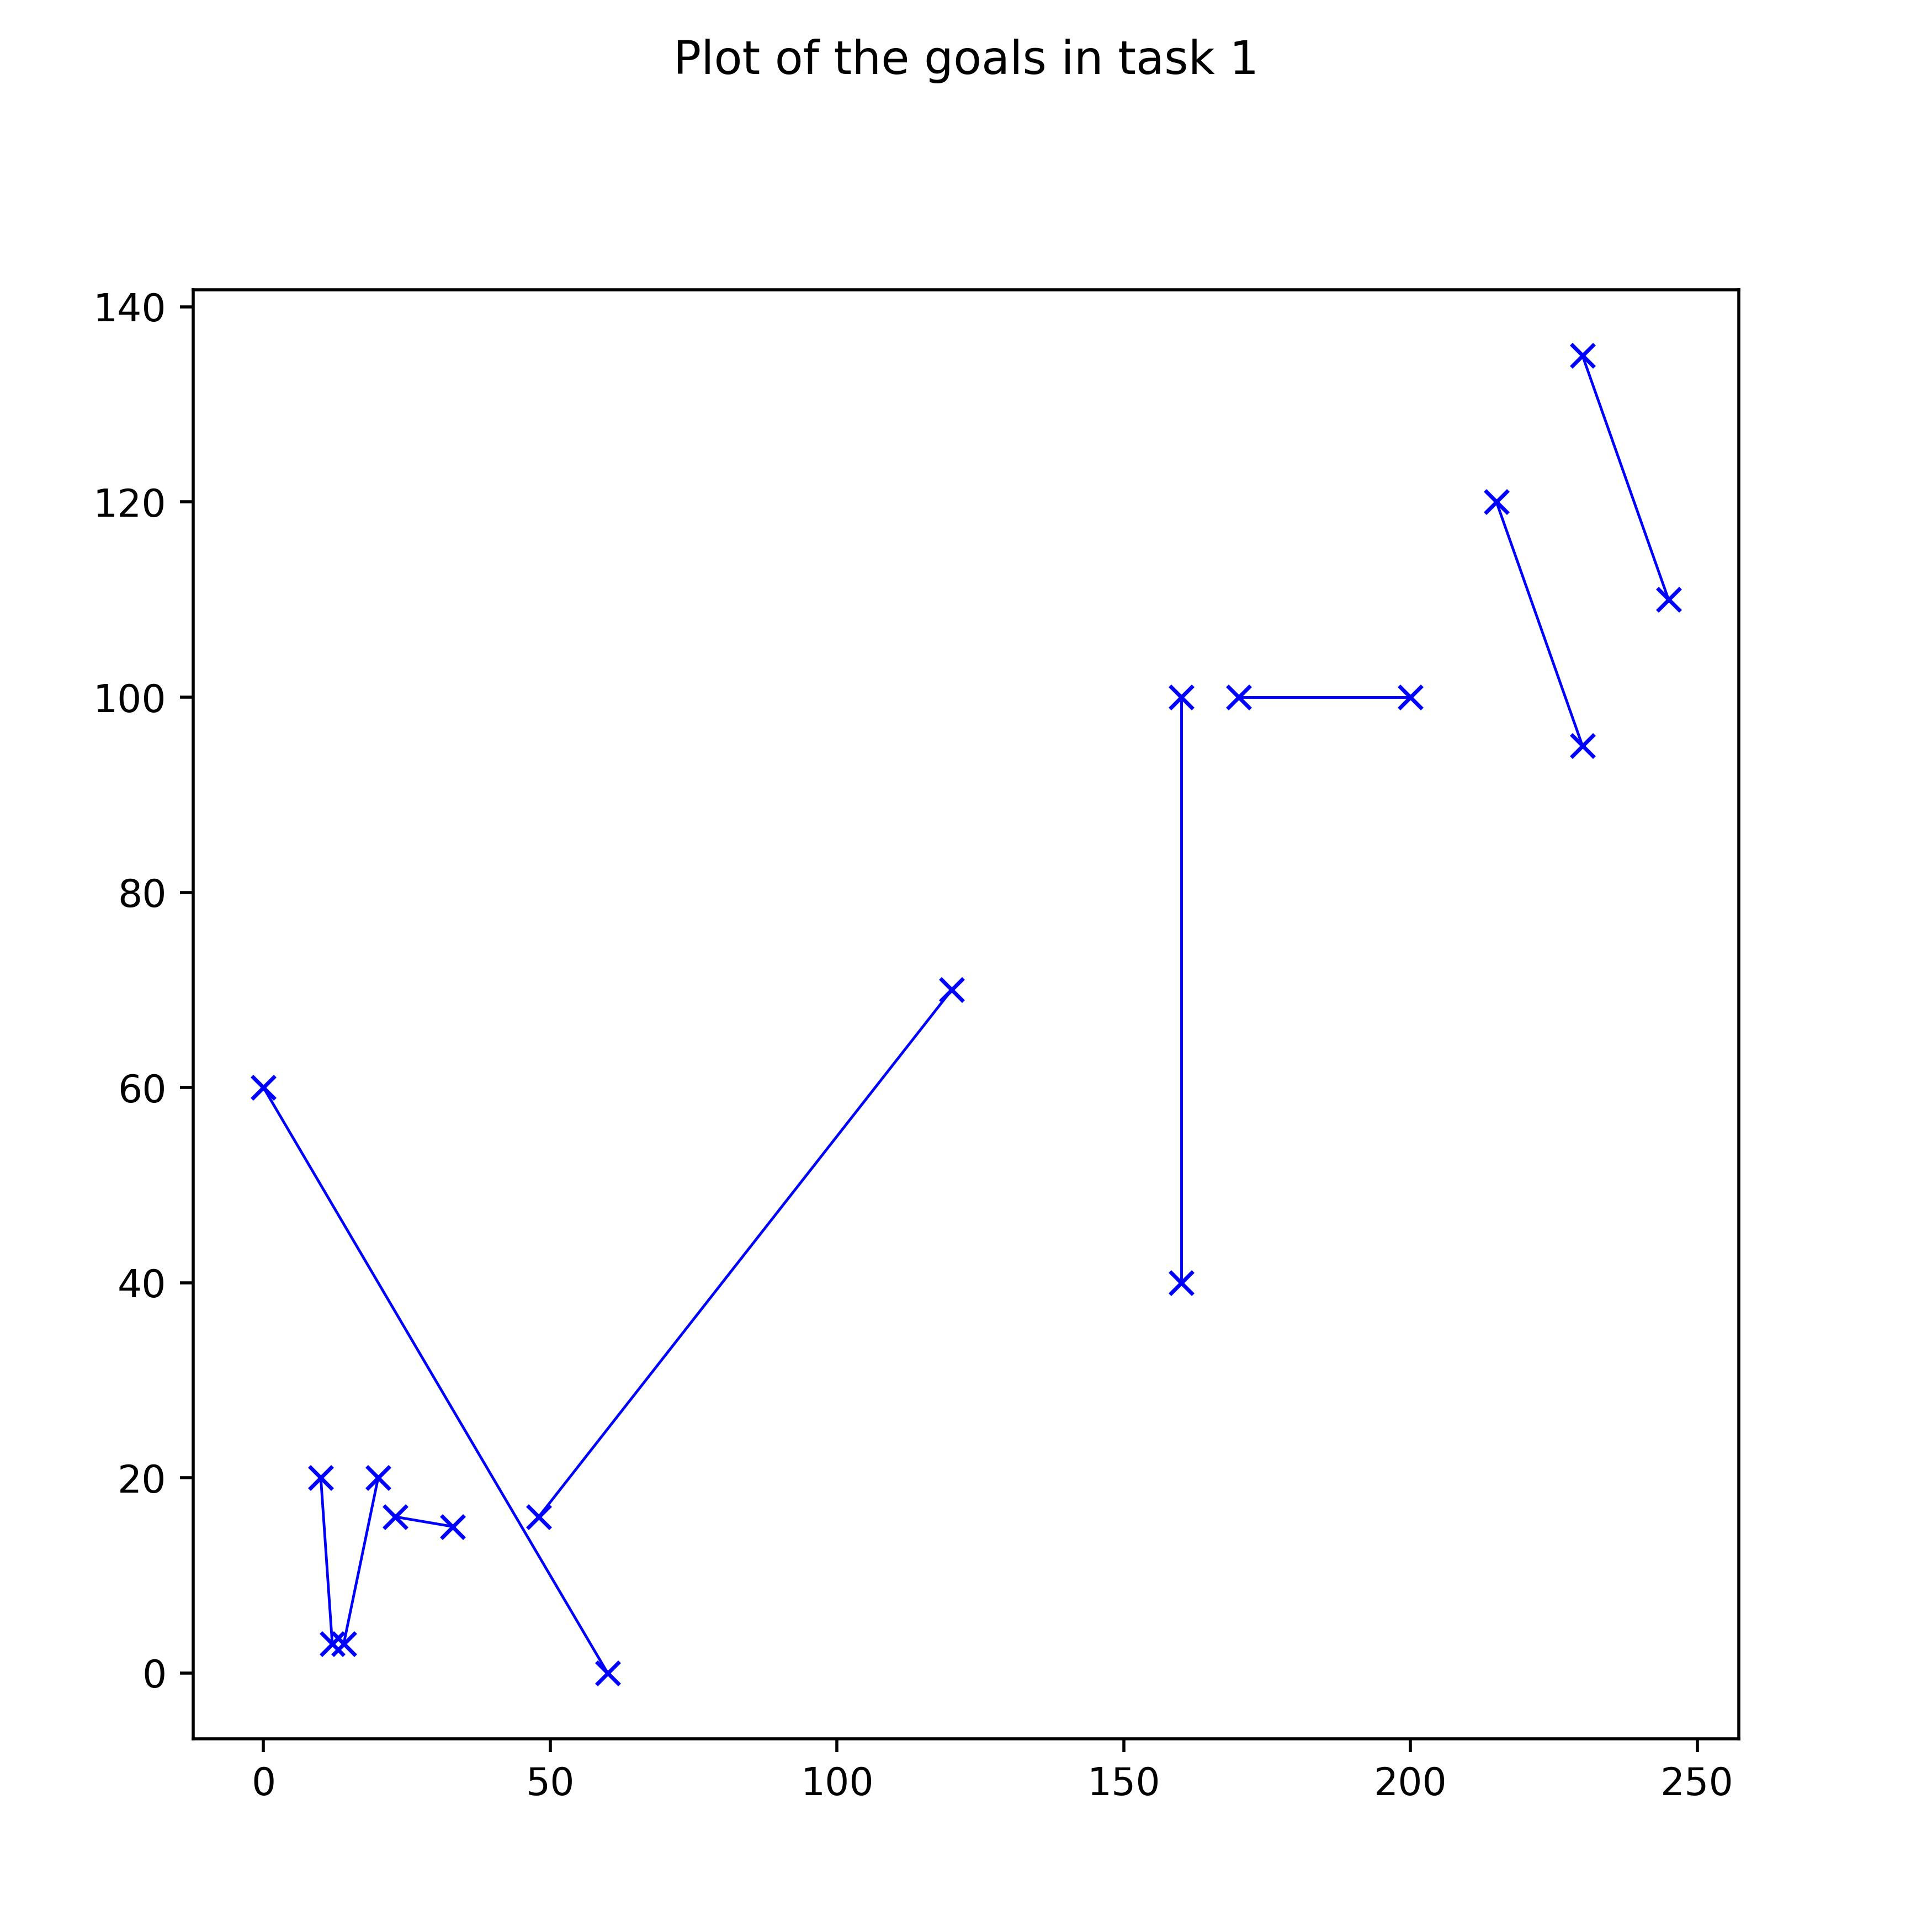
\includegraphics[width=\textwidth]{images/task_1.jpeg}
         \caption{Beispielaufgabe 1}
         \label{fig:y equals x}
     \end{subfigure}
     \hfill
     \begin{subfigure}[b]{0.49\textwidth}
         \centering
         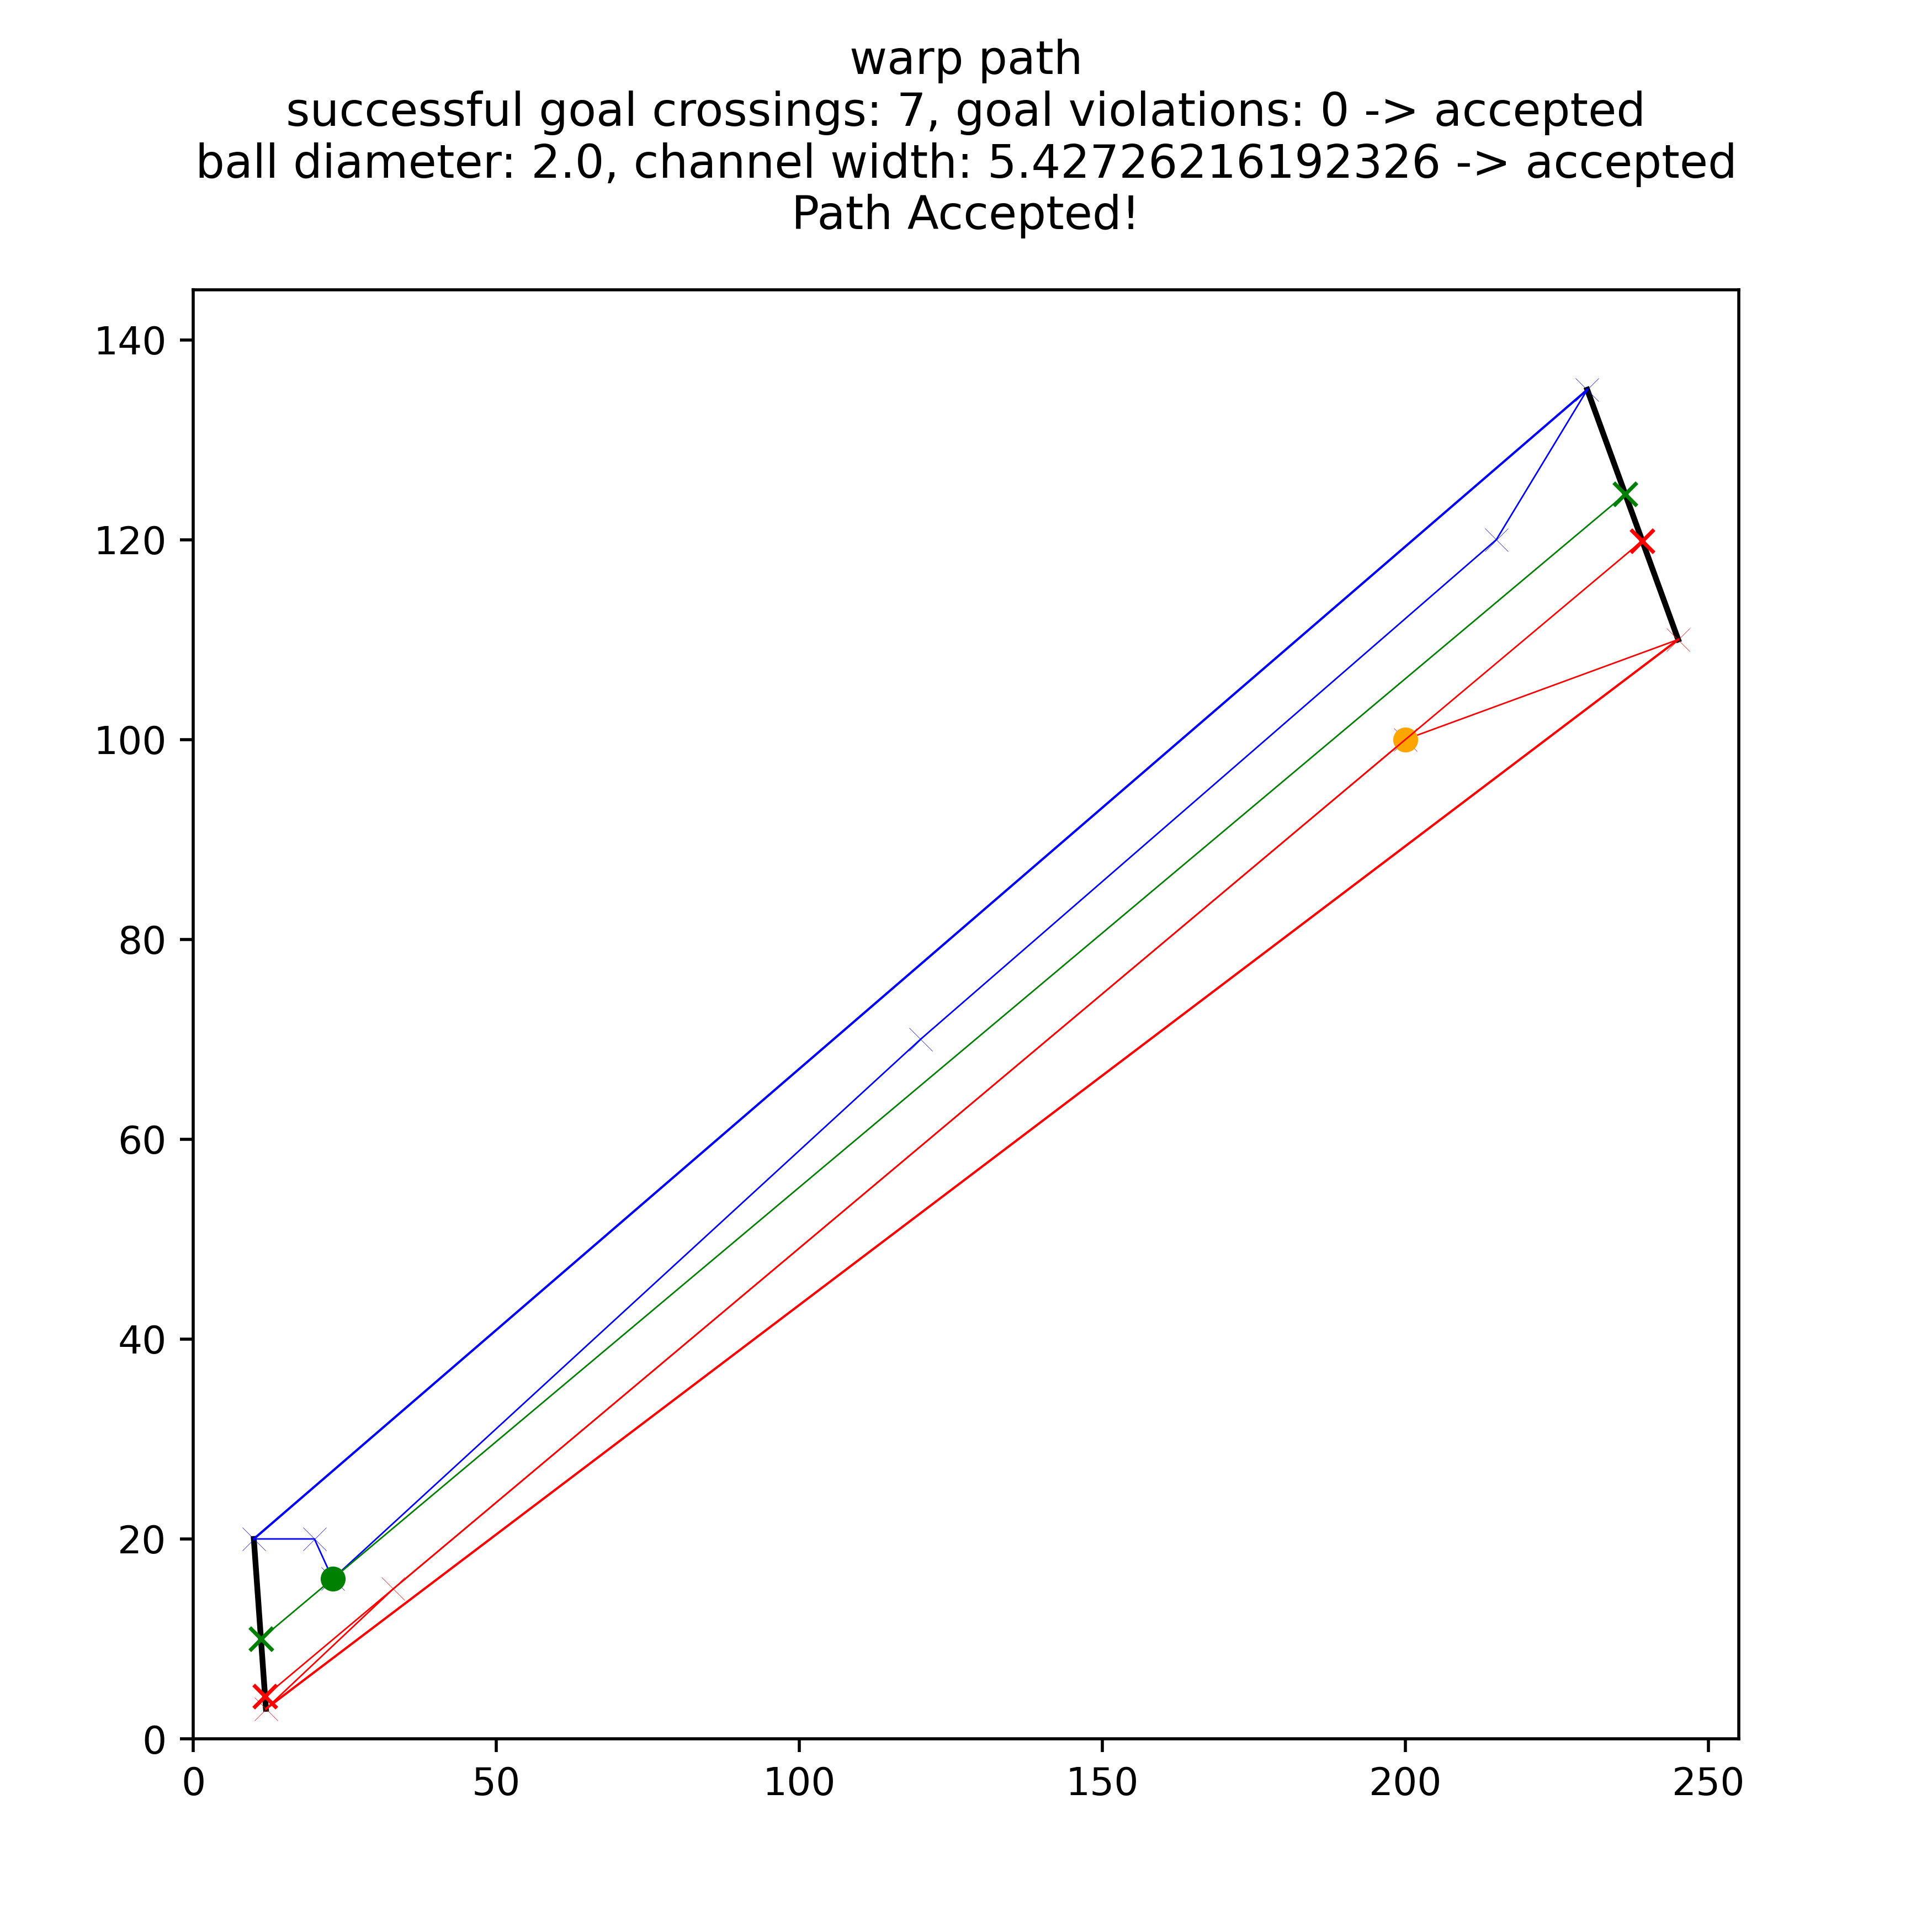
\includegraphics[width=\textwidth]{images/solution_task_1.png}
         \caption{Lösung der Beispielaufgabe 1}
         \label{fig:three sin x}
     \end{subfigure}
     \caption{Plot der Beispielaufgabe 1 und ihrer Lösung.}
        \label{fig:three graphs}
\end{figure}

\begin{figure}
\label{fig:beispiele2}
\vspace{-0.5cm}
\centering
     \begin{subfigure}[b]{0.49\textwidth}
         \centering
         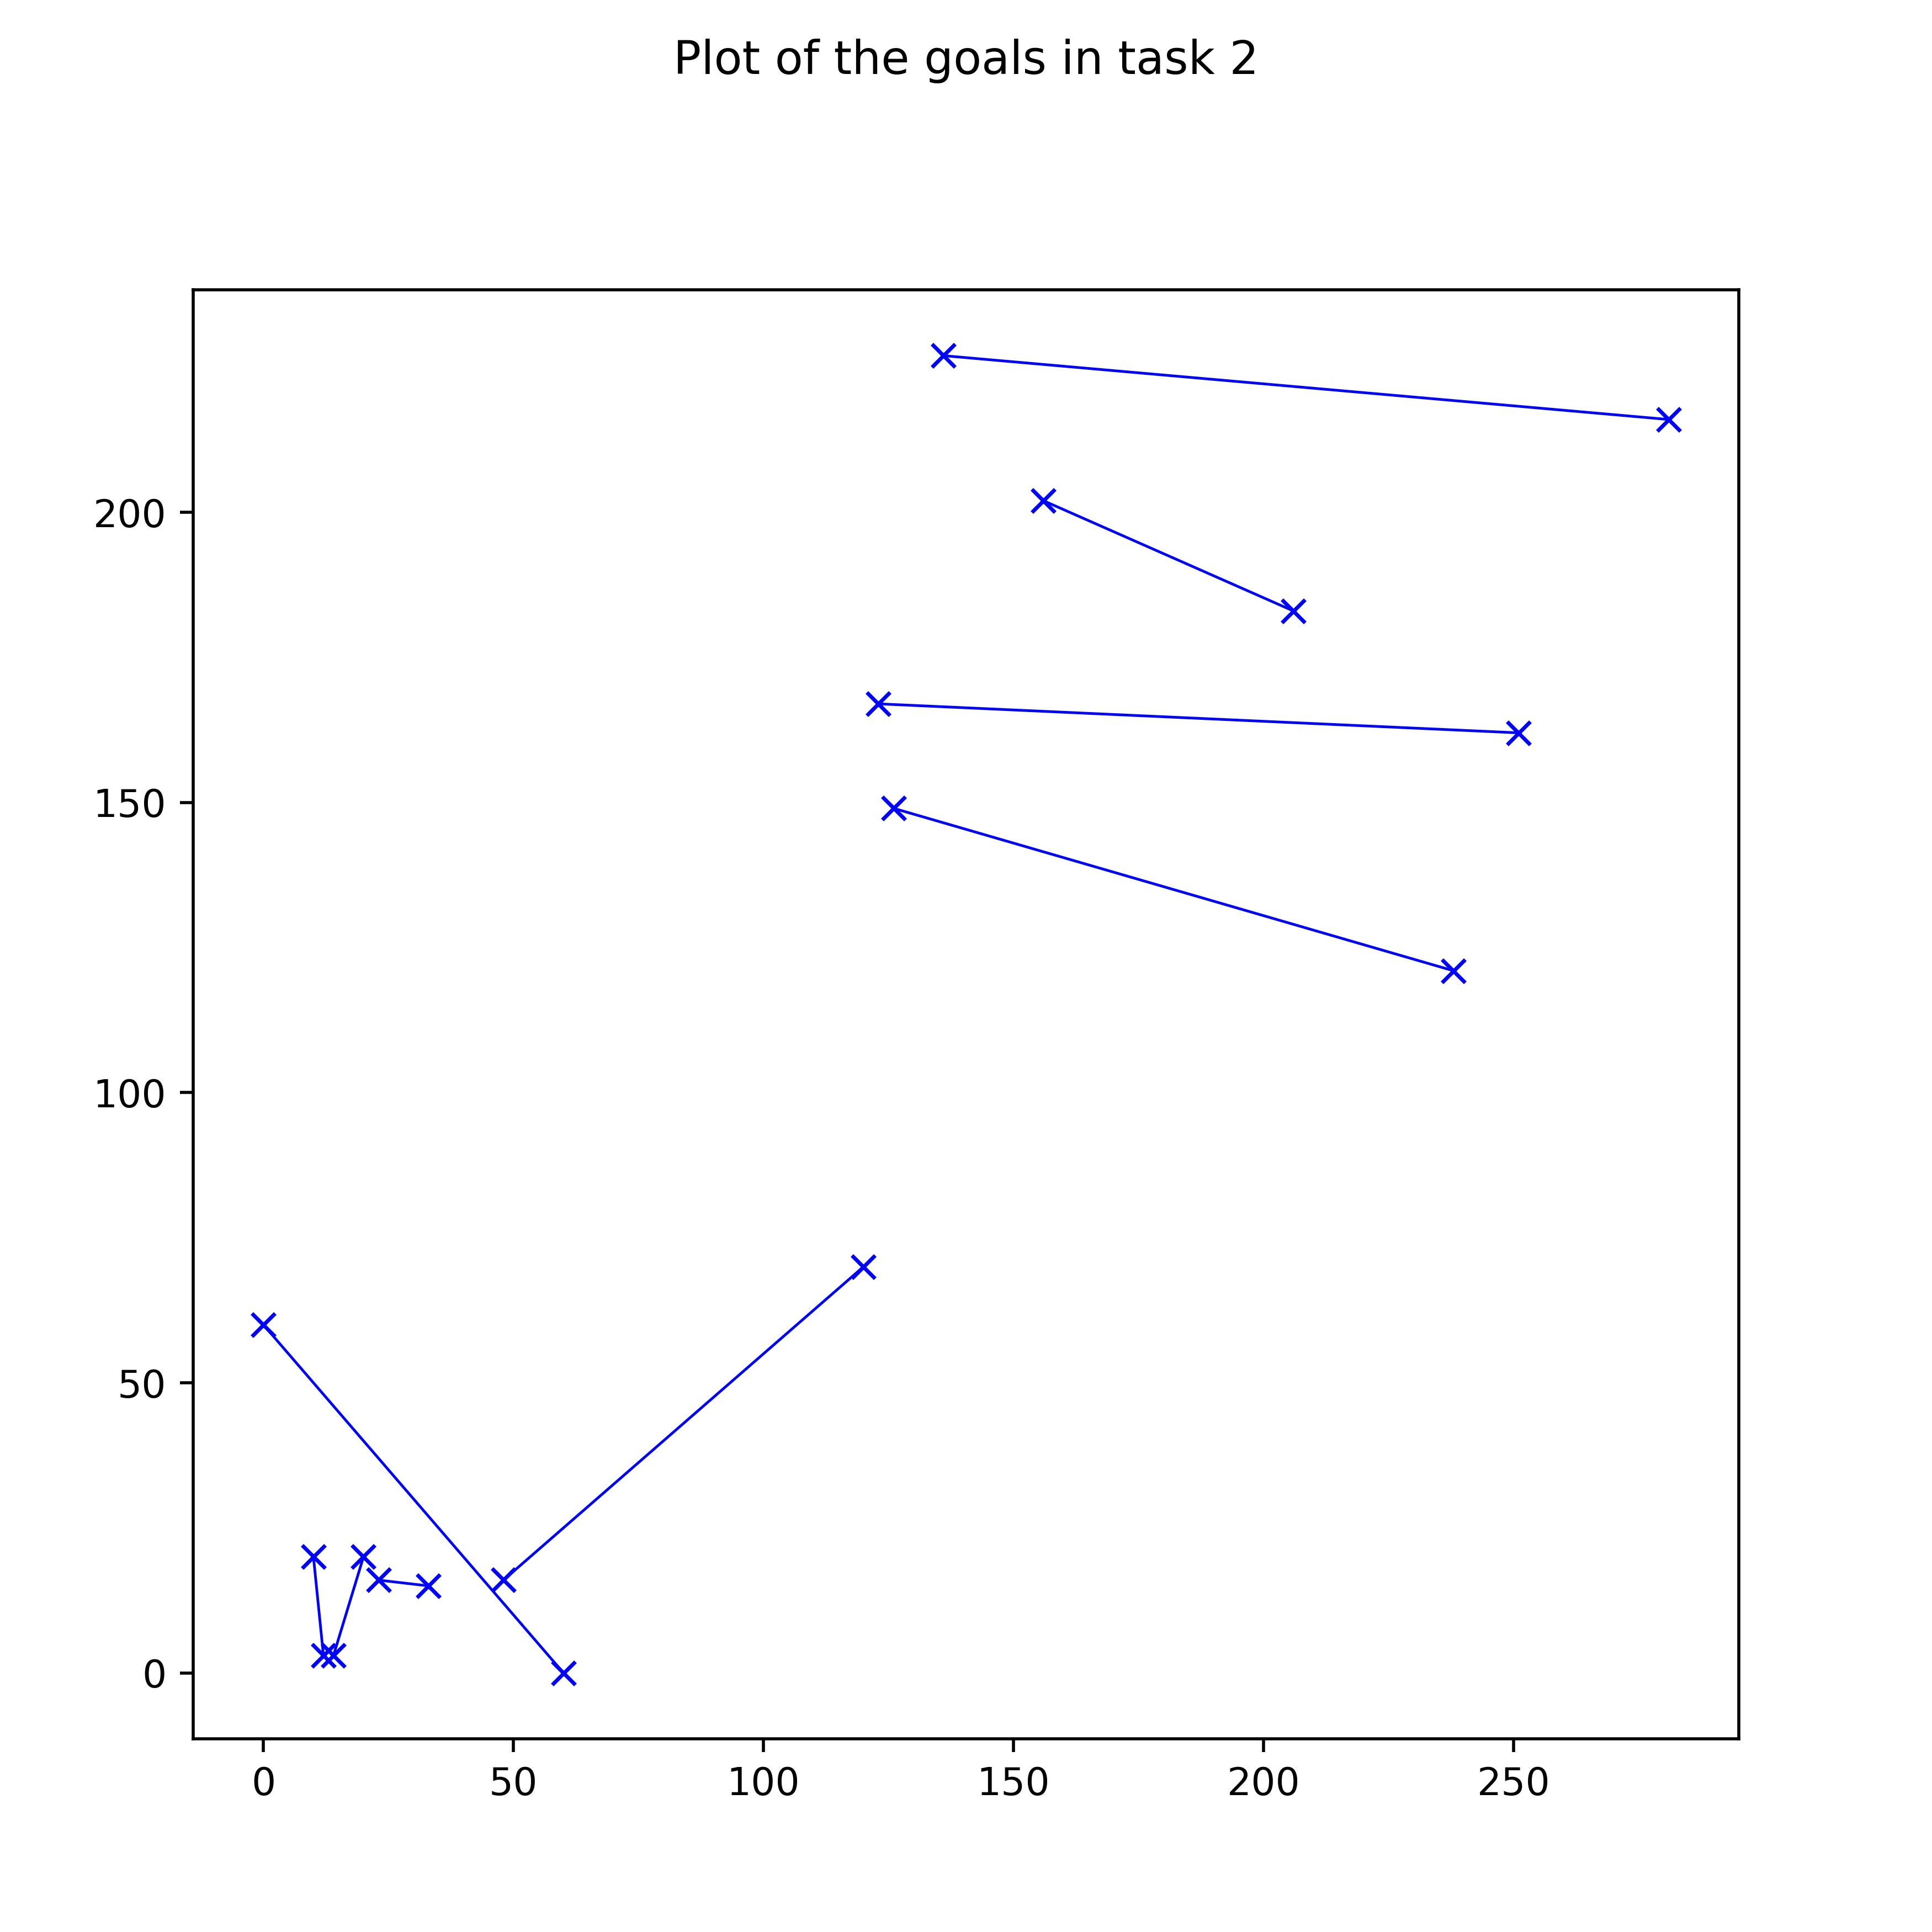
\includegraphics[width=\textwidth]{images/task_2.jpeg}
         \caption{Beispielaufgabe 2 besitzt keine Lösung, da es nicht möglich ist durch alle Tore zu schießen.}
         \label{fig:five over x}
     \end{subfigure}
     \hfill
     \begin{subfigure}[b]{0.49\textwidth}
         \centering
         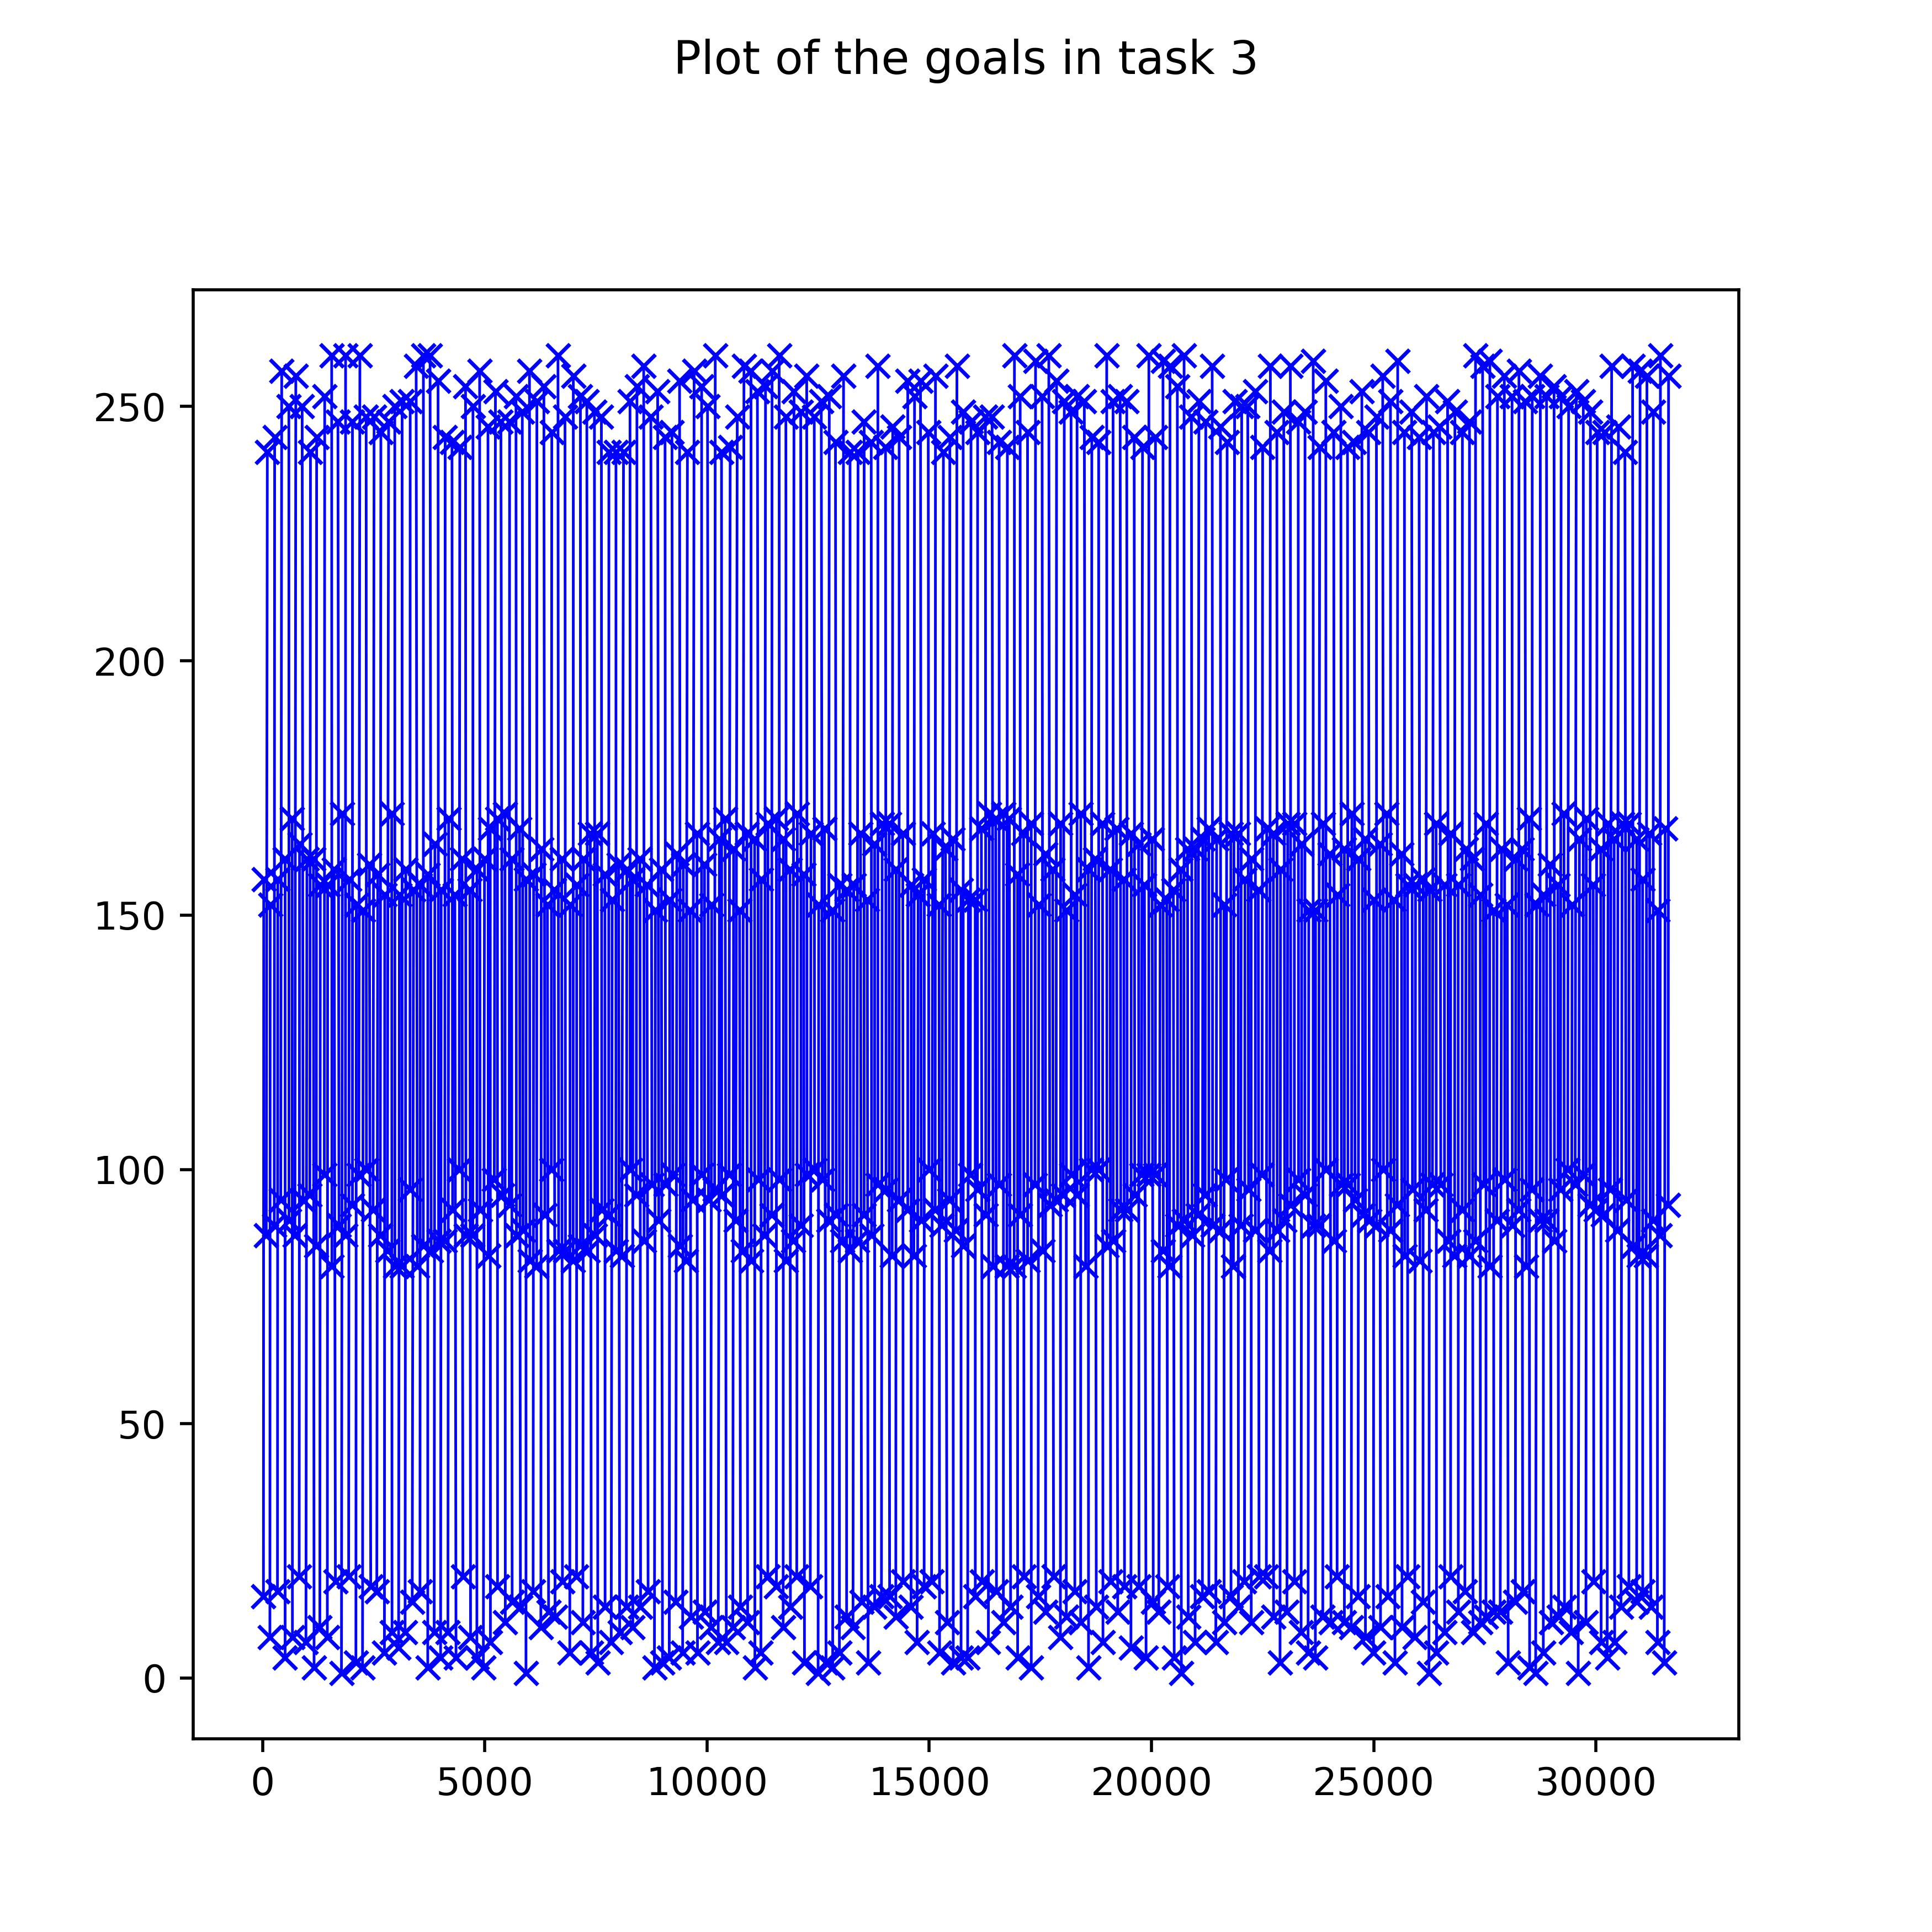
\includegraphics[width=\textwidth]{images/task_3.jpeg}
         \caption{Beispielaufgabe 3 besitzt keine Lösung, da die Tore in der falschen Reihenfolge sind.}
         \label{fig:five over x}
     \end{subfigure}
     \hfill
     \begin{subfigure}[b]{0.49\textwidth}
         \centering
         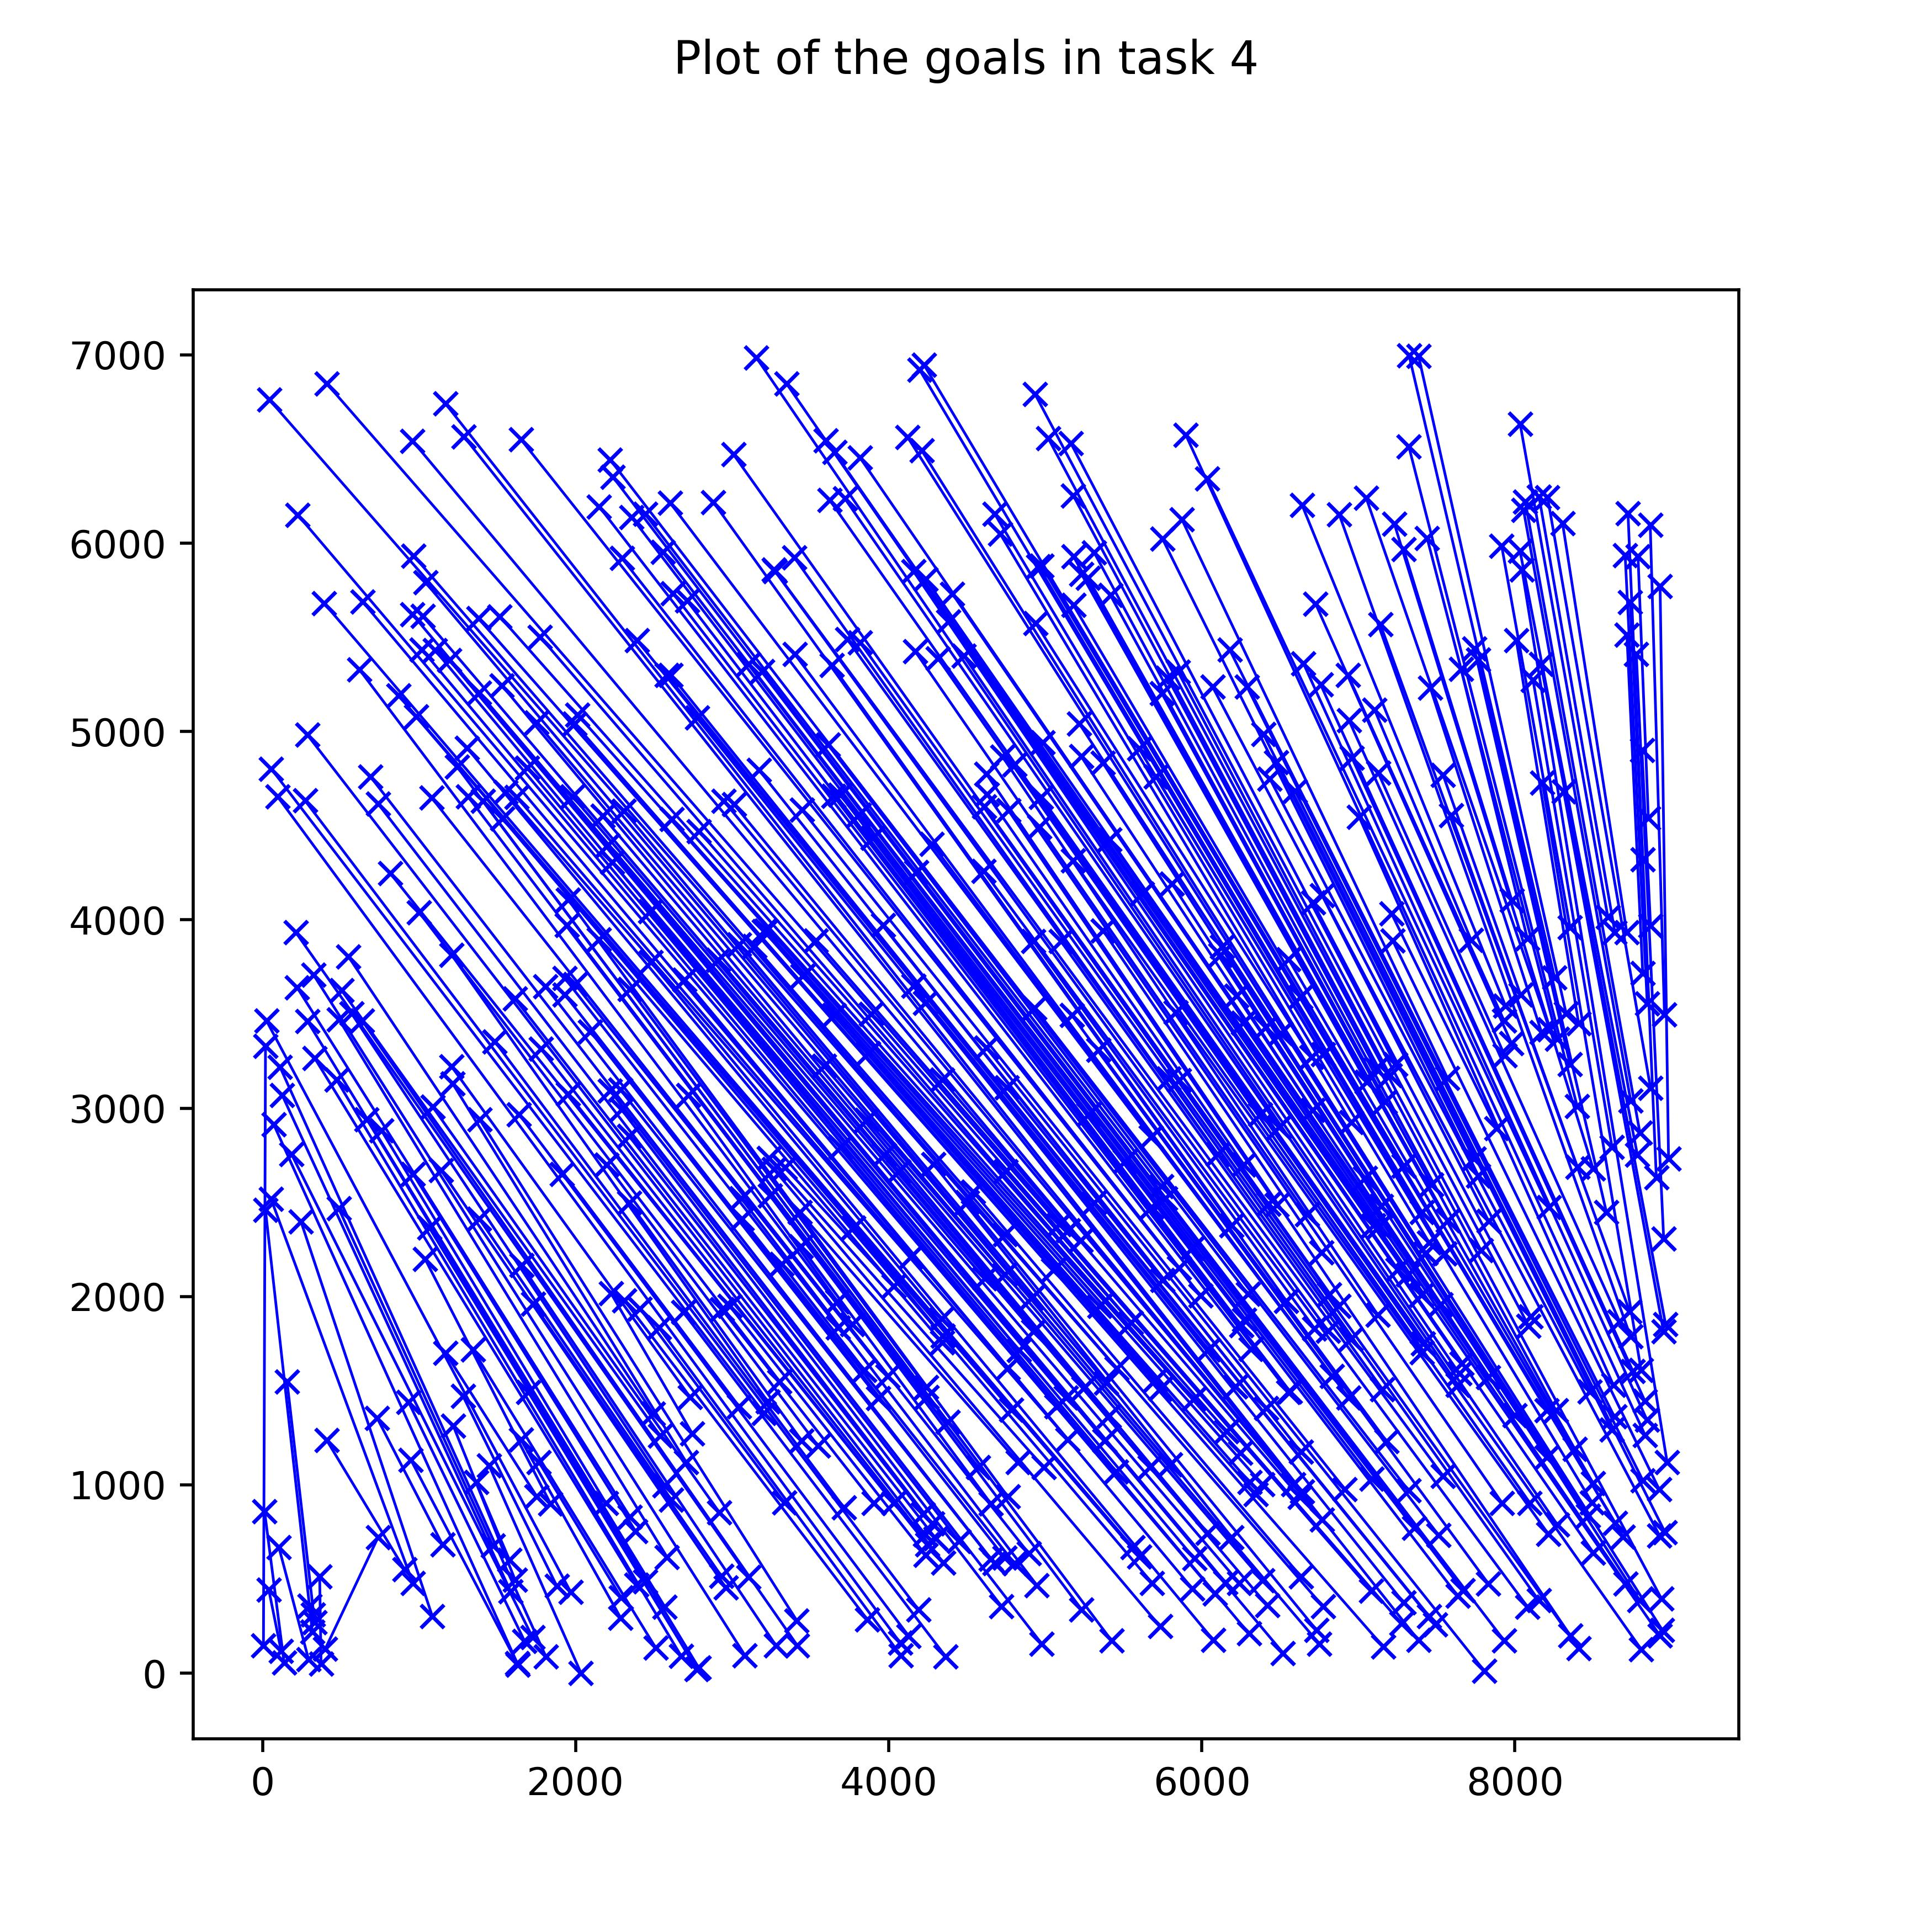
\includegraphics[width=\textwidth]{images/task_4.jpeg}
         \caption{Beispielaufgabe 4}
         \label{fig:five over x}
     \end{subfigure}
     \hfill
     \begin{subfigure}[b]{0.49\textwidth}
         \centering
         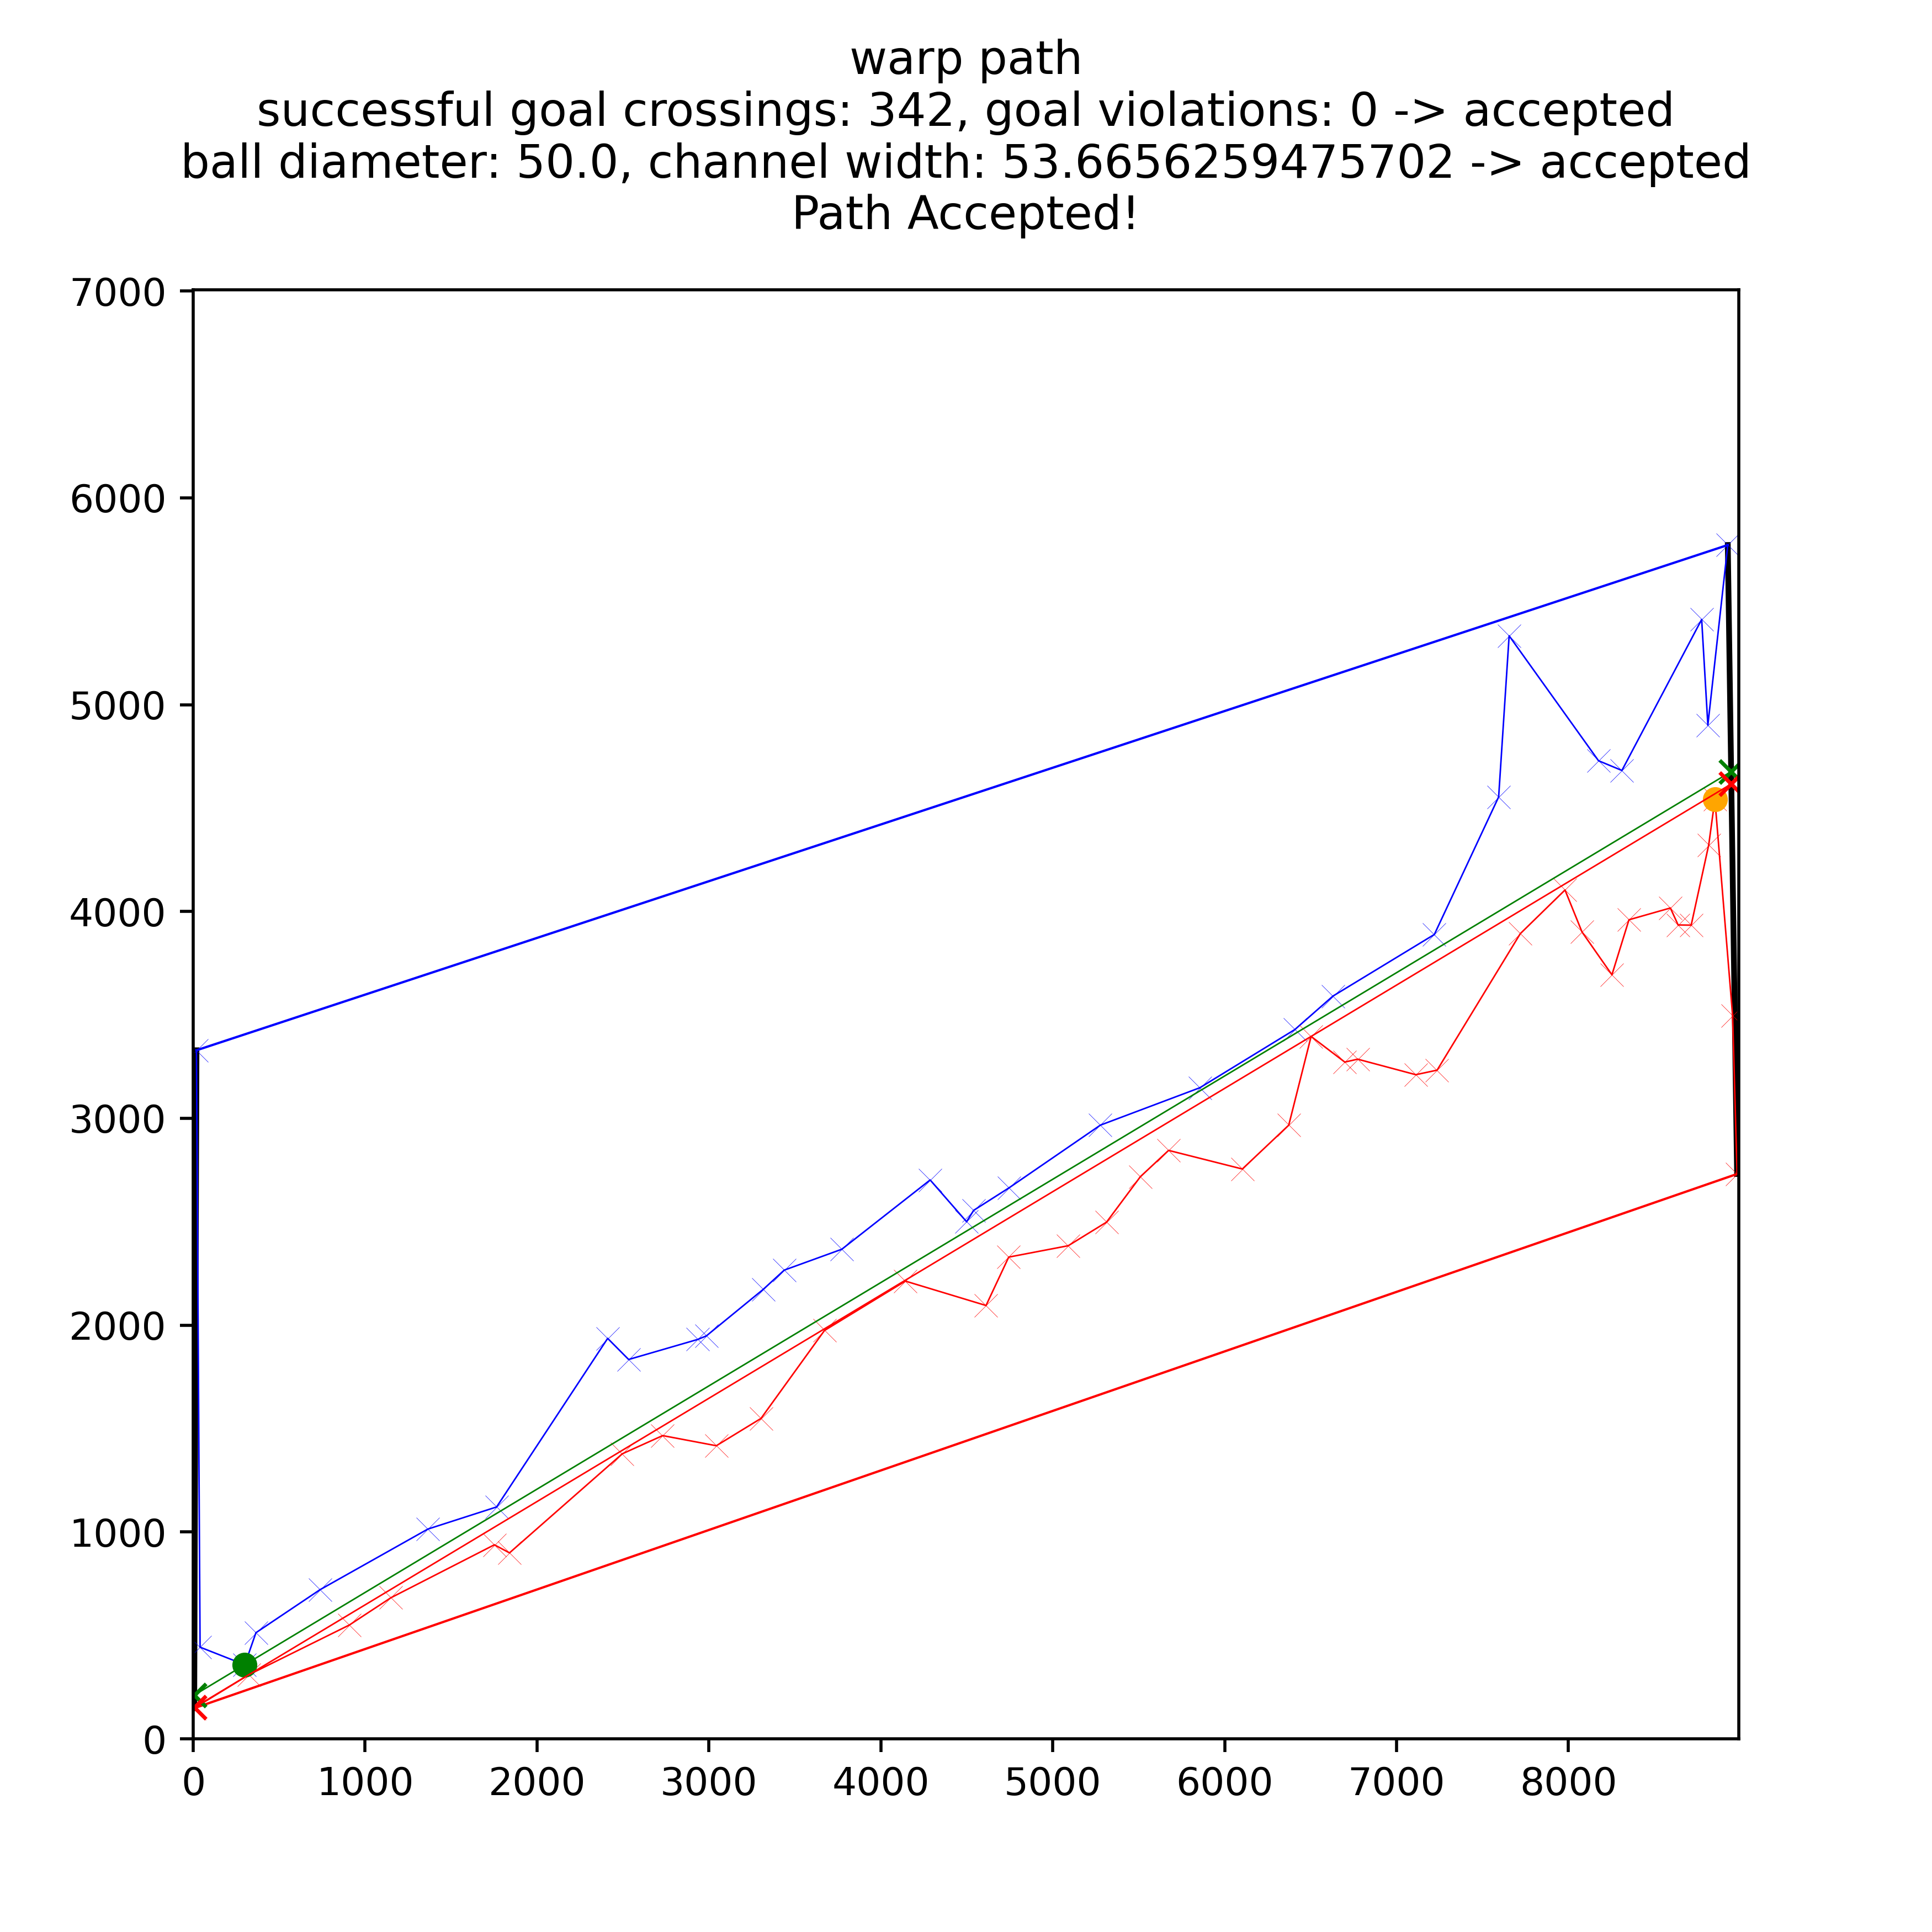
\includegraphics[width=\textwidth]{images/solution_task_4.png}
         \caption{Lösung der Beispielaufgabe 4}
         \label{fig:five over x}
     \end{subfigure}
          \hfill
     \begin{subfigure}[b]{0.49\textwidth}
         \centering
         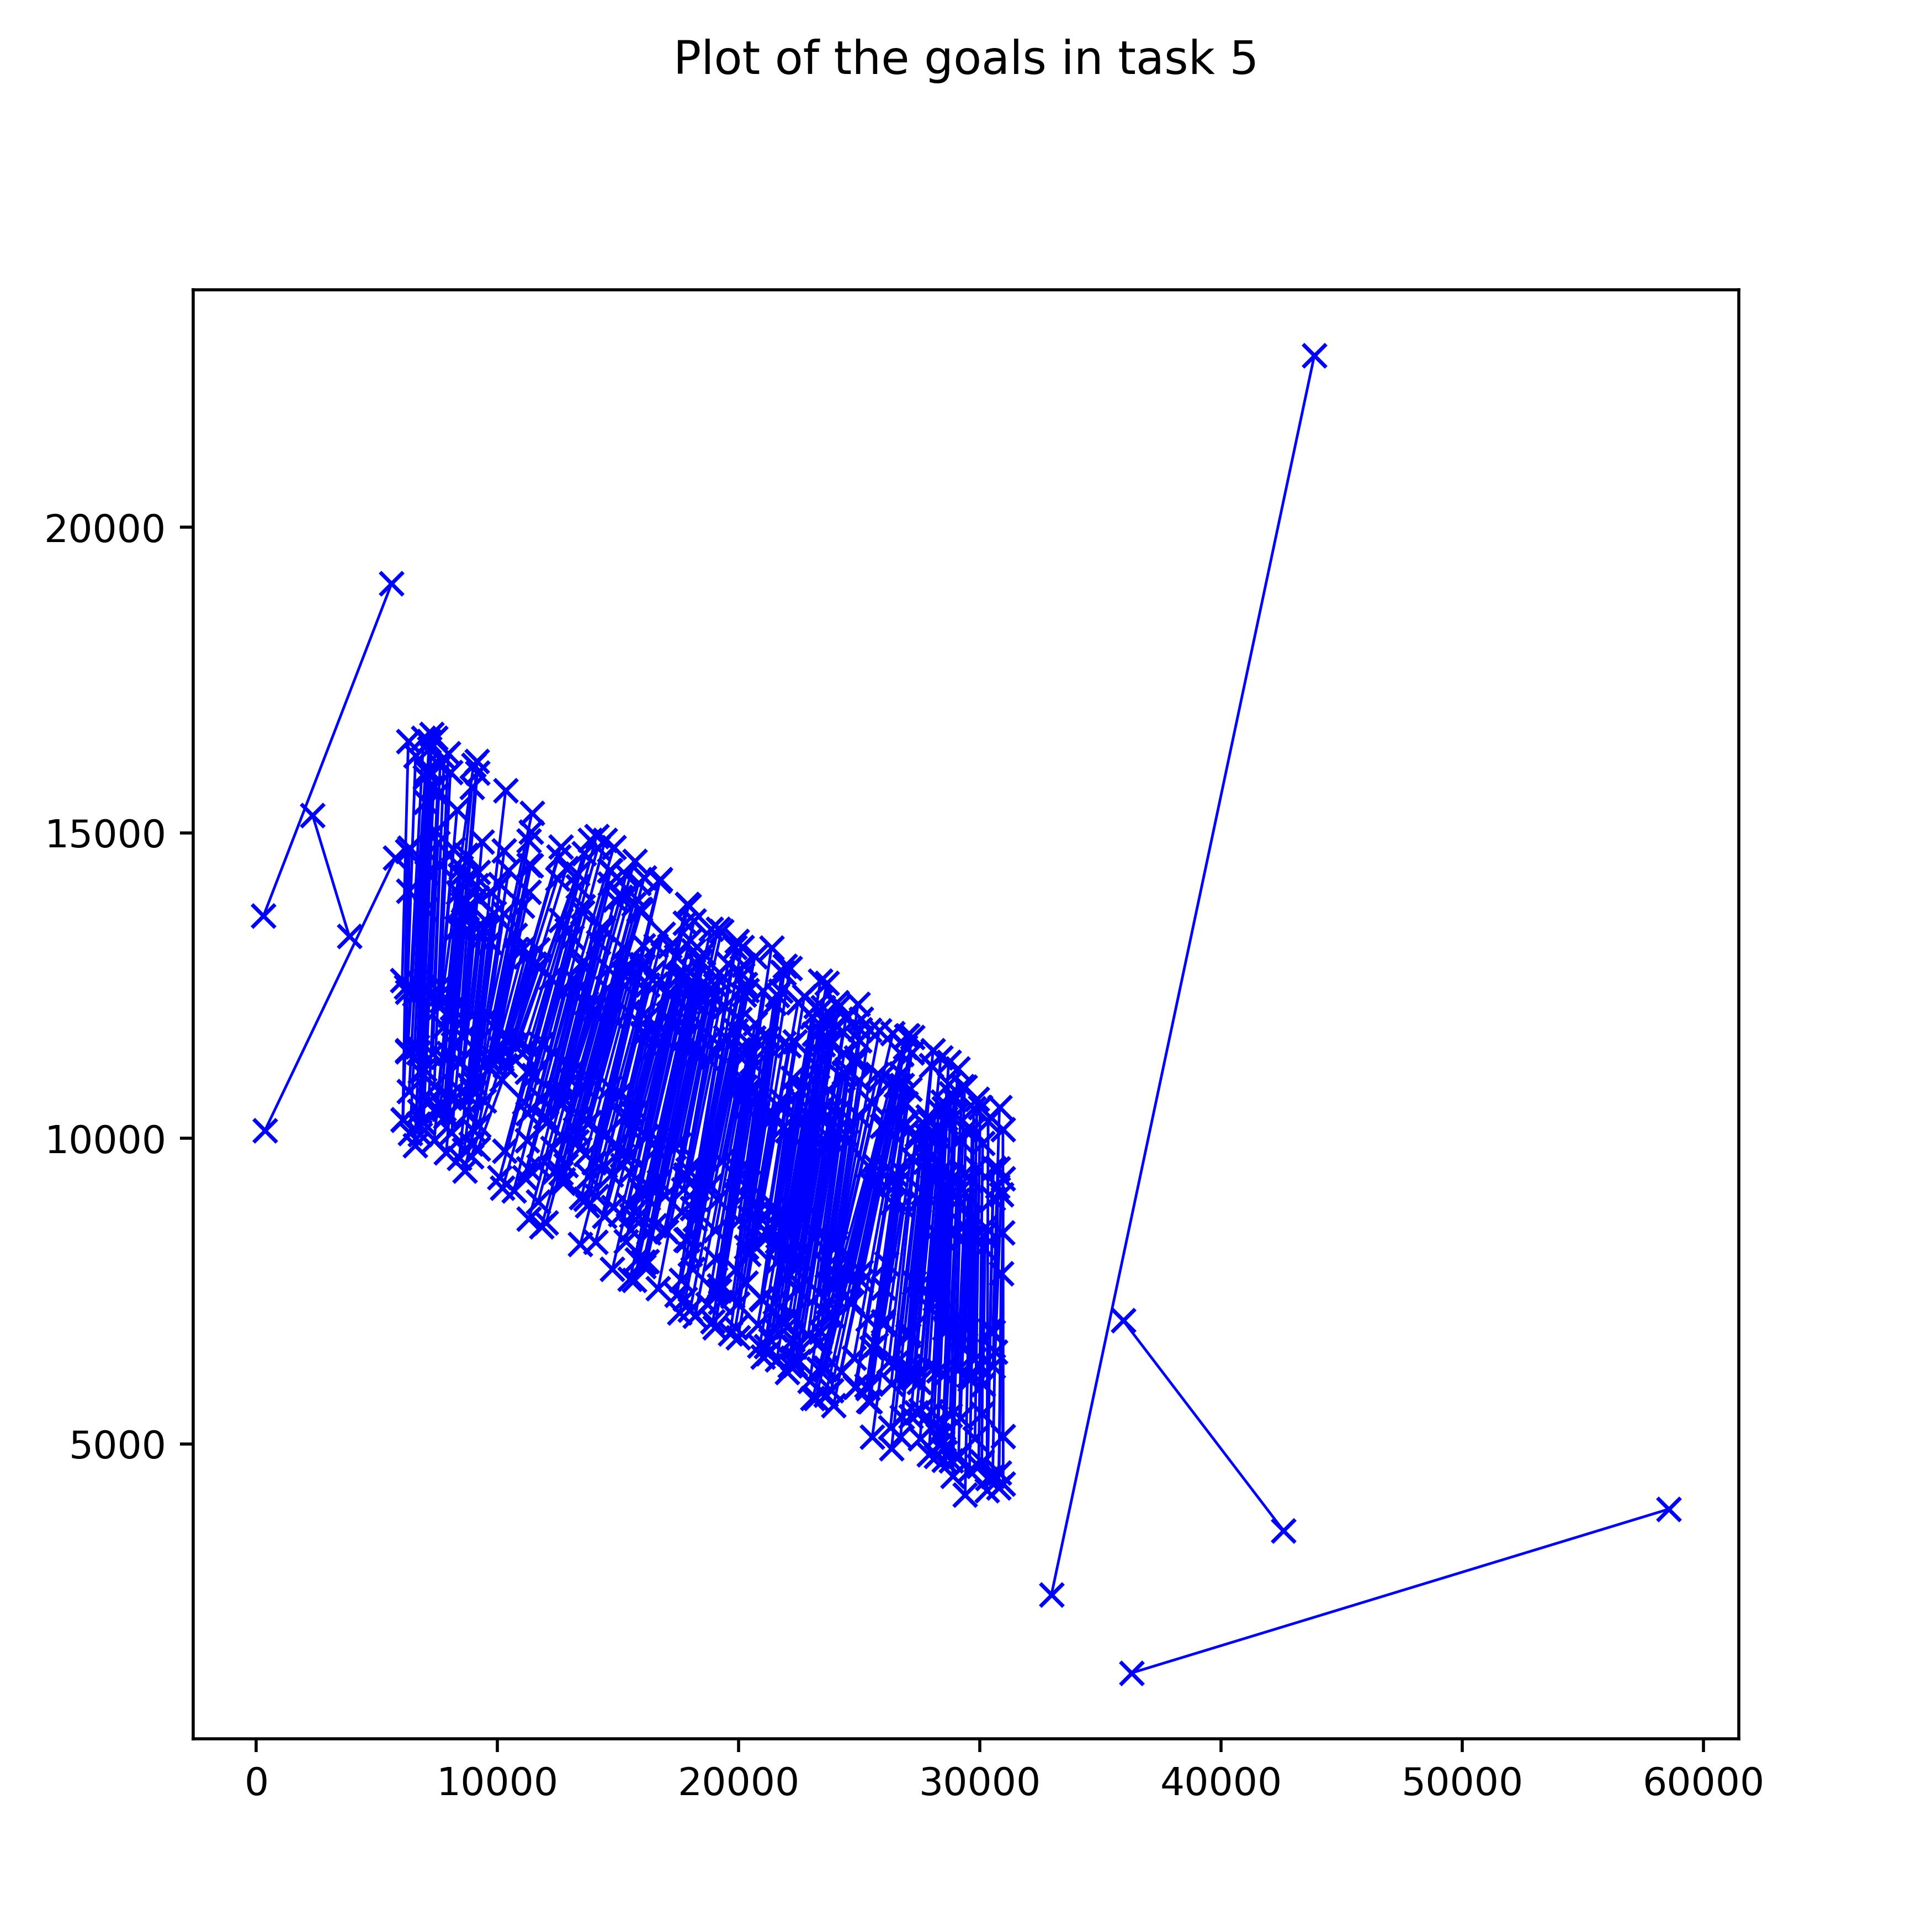
\includegraphics[width=\textwidth]{images/task_5.jpeg}
         \caption{Beispielaufgabe 5}
         \label{fig:five over x}
     \end{subfigure}
     \hfill
     \begin{subfigure}[b]{0.49\textwidth}
         \centering
         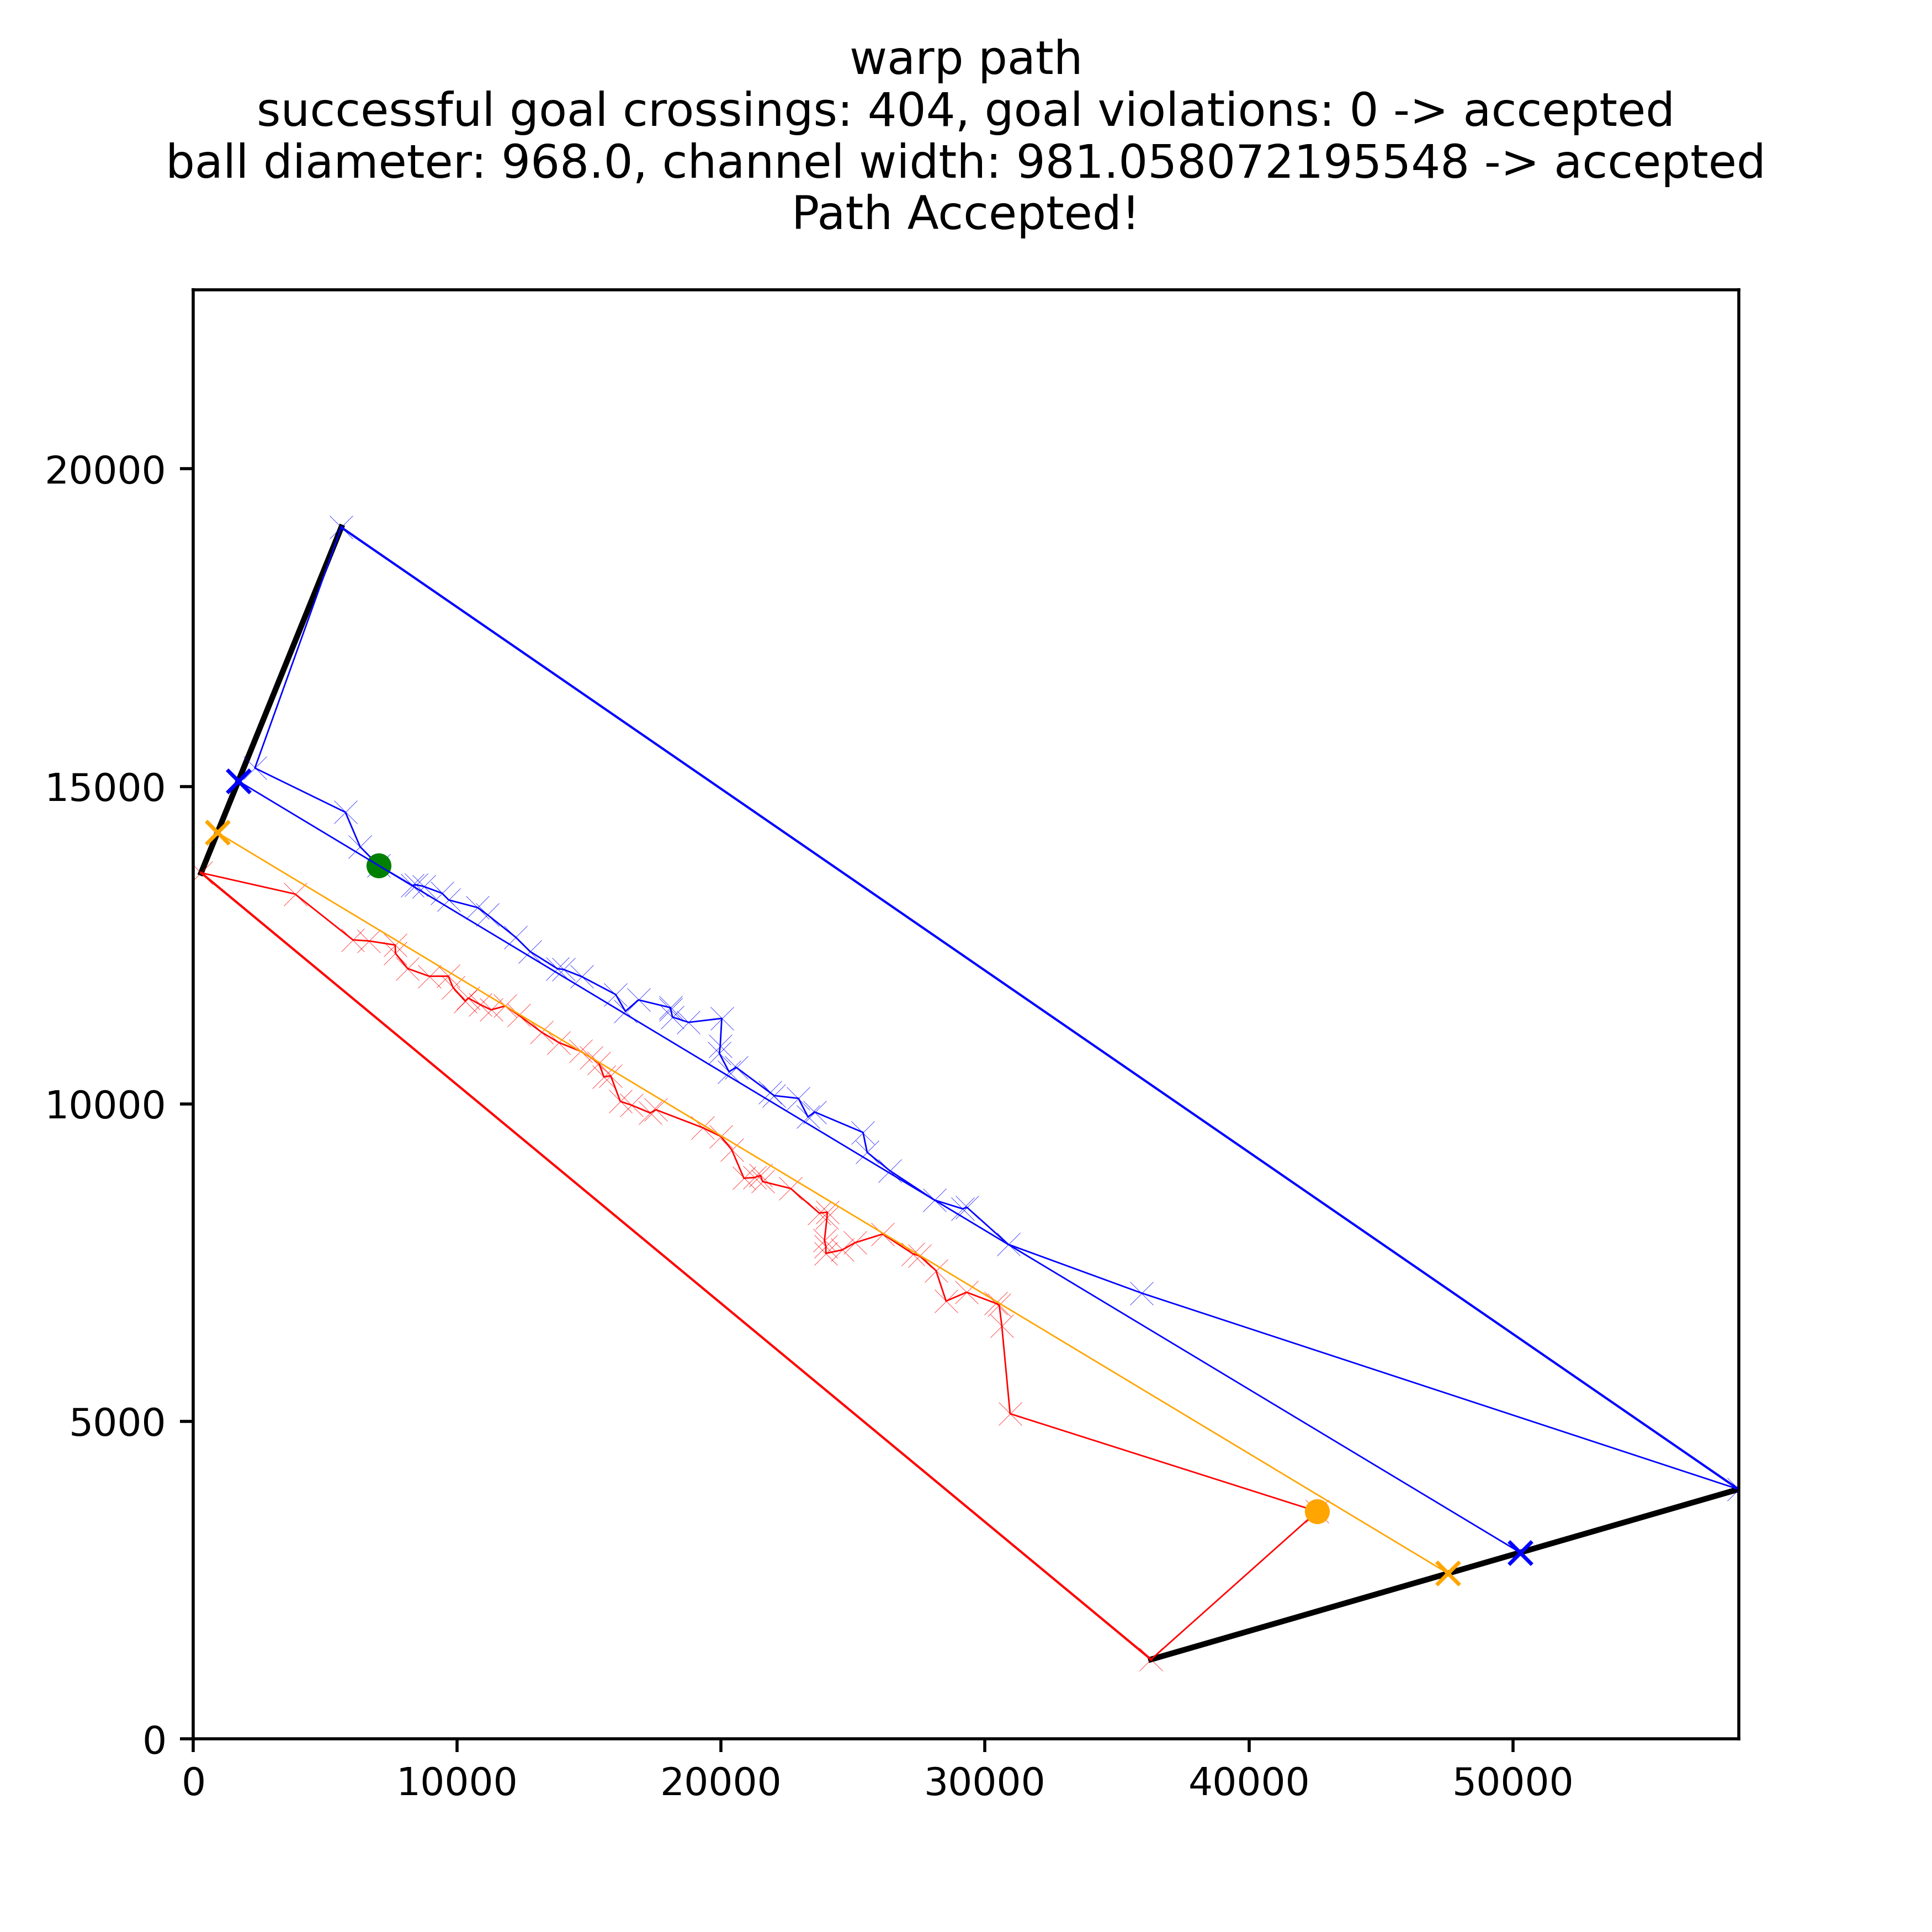
\includegraphics[width=\textwidth]{images/solution_task_5.png}
         \caption{Lösung der Beispielaufgabe 5}
         \label{fig:five over x}
     \end{subfigure}
        \caption{Plots der Beispielaufgaben 2 bis 5 und ihrer Lösung, sofern eine Lösung existert.}
        \label{fig:three graphs}
\end{figure}

